\documentclass{../../../ksp}

\title{KSP 36--3--2}
\author{Daniel Culliver}
\date{February 2024}

\usepackage{babel}

\begin{document}

\maketitle

\section*{Introduction}

First, we will define the keyword \emph{``collapse''}, to define the combination of and both of its children.
If the children themselves aren't collapse, then the collapse of tha parent encompasses the collapse of its children.
With this recursive action, we can simply say, that the problem we are solving is how to collapse the root node of the tree with the least amount of memory possible.

Another thing to note, is that when we start the collapse of, for example, the left child of a node, then no matter at which step we are, we will be taking up some memory.
It stands to reason, that once we collapse a node, then we will want to complete its collapse, before we move onto the next node.
Together with the recursive nature of our ``collapse'', the answer of the problem will look rather similar to the order we leave nodes when traversing a tree recursively, except that we will have a given start.

\begin{figure}[H]
    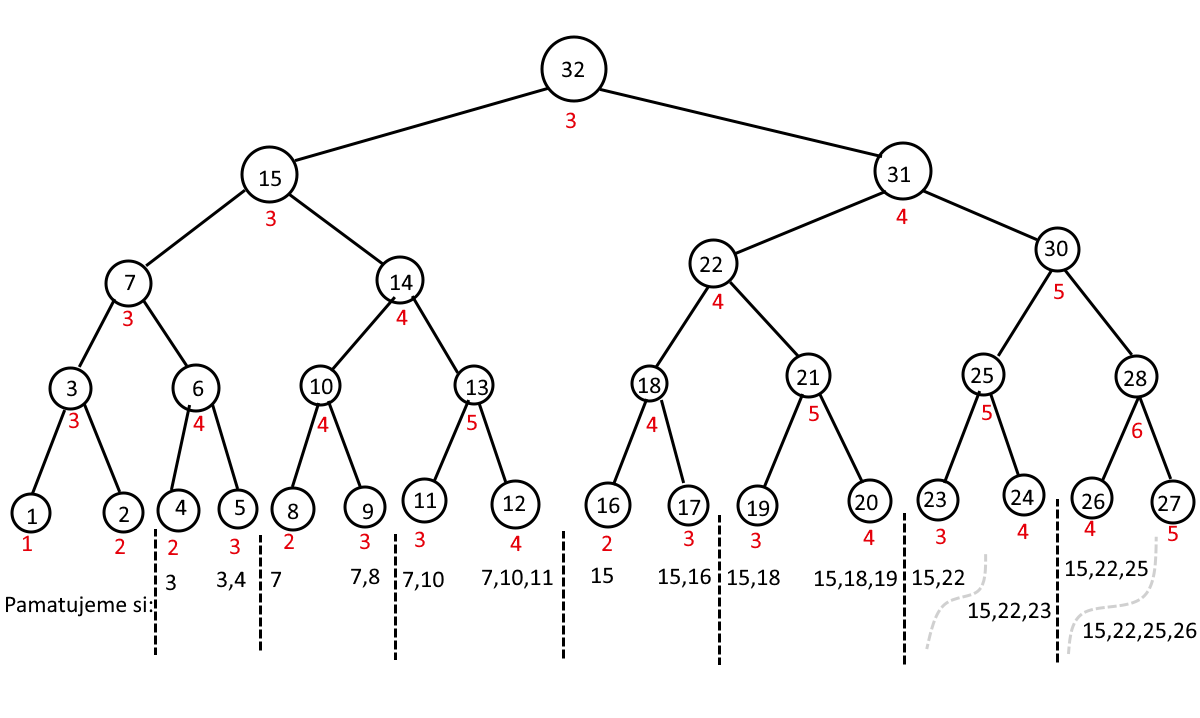
\includegraphics[width=\textwidth]{./base example.png}
\end{figure}

The example above shows a tree with its nodes numbered according the the order we would write them out in the answer.
The red number below the nodes indicate the memory taken up by the algorithm at the final moment of the collapse of that node.
We also included the nodes in the memory during the selection of any leaf, so as to help the reader understand why the cost is higher.
The picture perfectly shows, that the base price of the collapse of a node with two children is 3, and that this price is increased when we collapsed a neighbouring subtree first.

\section*{Algorithm}

Now, for the algorithm itself, we will introduce another example tree, this one being asymmetrical:

\begin{figure}[H]
    \centering
    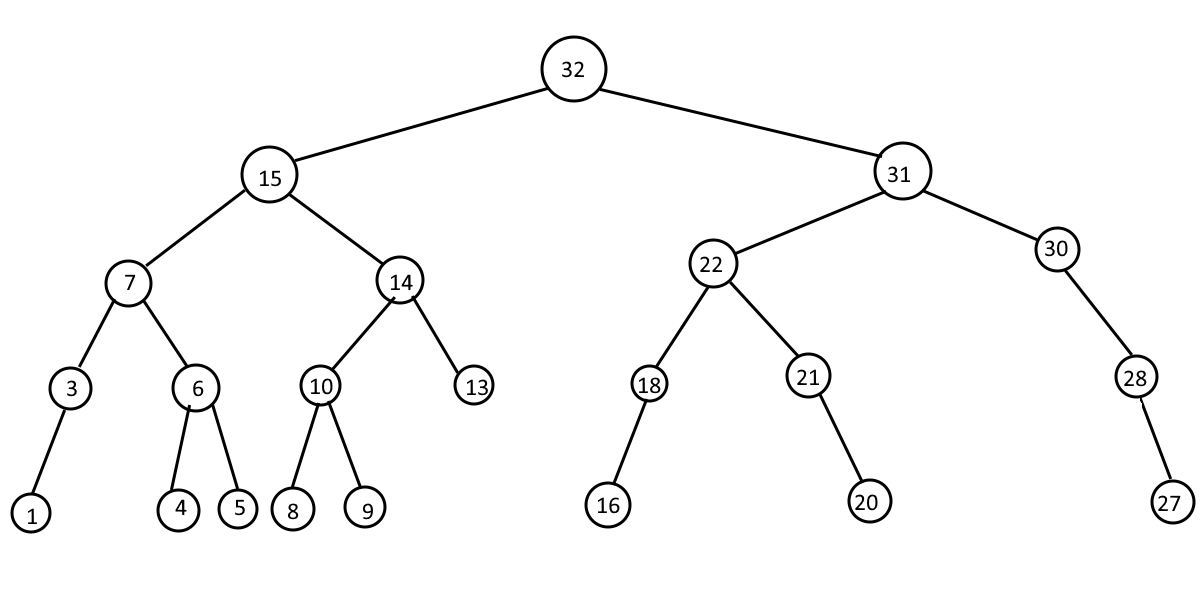
\includegraphics[width=\textwidth]{./asym example base.png}
\end{figure}

First off, we the numbers no longer define the order of the nodes and instead will just be their IDs, because I placed them in the wrong drawing layer.
With the first example we know, that we will want to start at the node, which could potentially become the most expensive one to collapse, because by starting with it, it won't reach a high price.
And so our first step will be to traverse the tree, saving the collapse price of each child node, as if we collapsed the other child first:

\begin{figure}[H]
    \centering
    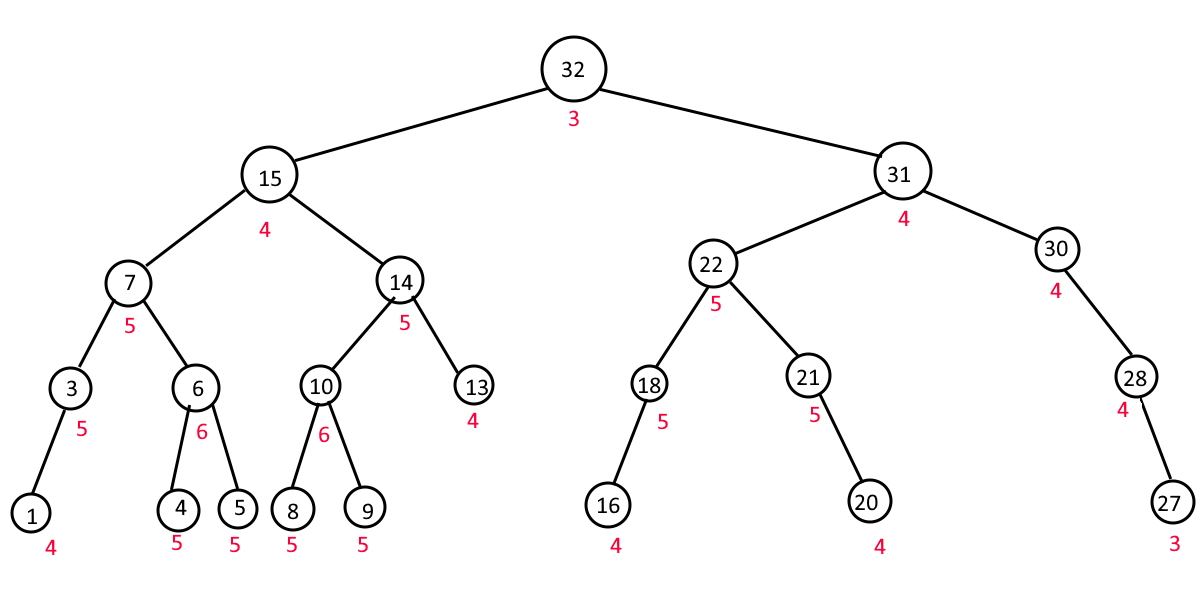
\includegraphics[width=\textwidth]{./asym example step 1.png}
\end{figure}

Here we can clearly see, that each time a node has two children, the price increases, if the node has one child, the price stays the same, and if the node is a leaf, then the price decreases.
We can also see which nodes have the highest potential price, in other words the nodes we will want to start with.

The next step of the algorithm is the reduction of the prices.

Since the calculation of the highest costs can end at any leaf, we will start the reduction from the root of the tree.
It's clear that we will want to reduce the left subtree first, because that's where the highest costs are.
From the root node itself, it's impossible to know where exactly the highest cost is.
To solve this, all we need to do is modify the original recursive tree traversal, so that it not only calculates the highest price for each node, but also saves the most expensive price of any of its descendants.
This modification doesn't increase the time complexity of the tree traversal, keeping it $\BigO(N)$.

Now that each node knows its most expensive descendant, we can reduce the costs of the nodes by simply prioritising the expensive nodes above others.
It is also impertitent to mention, that since we are reducing from the top of the tree, a decrease in a node's cost signifies the reduction of the costs of all of its descendants (since this is just the inverse of calculating the highest cost).
Following these instructions, from the original highest cost state of the tree, we will first reduce node 15.
Next, both subtrees contain the same highest cost, so it doesn't matter which way we go, so we reduce node 7, and then following that, node 6, 5 and 4.
Here are the results:

\begin{figure}[H]
    \centering
    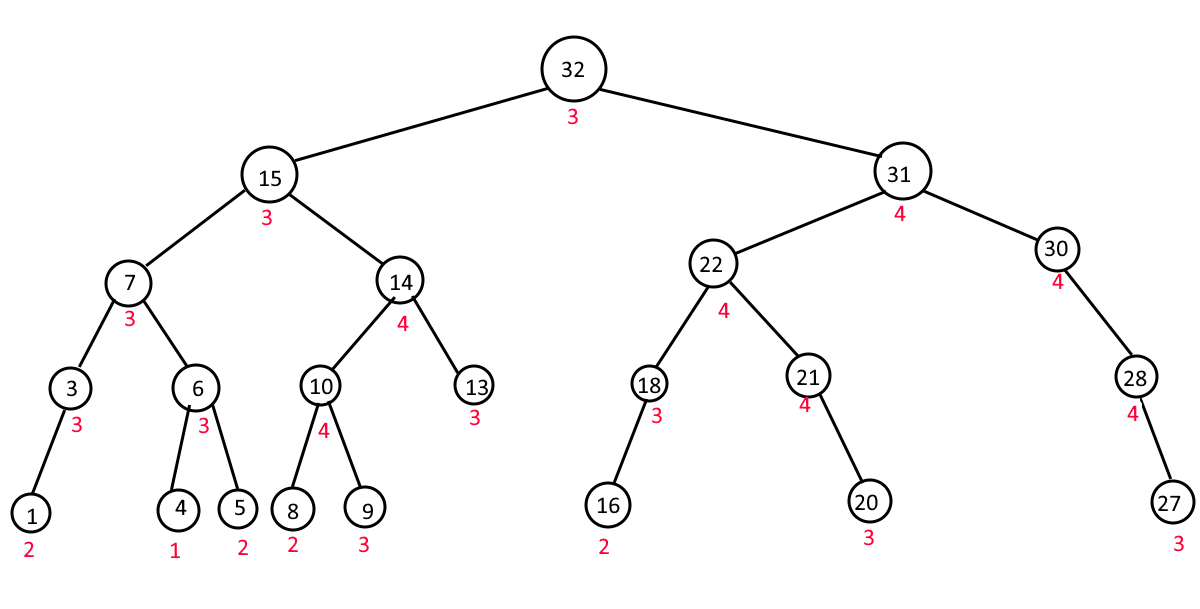
\includegraphics[width=\textwidth]{./asym example reduction.png}
\end{figure}

The costs of each node clearly indicate the order in which we will proceed, when actually collapsing the root node.
Because we start with the highest costs and subsequently reduce the most expensive nodes, we can be assured, that the discovered solution is lowest maximum cost, thus solving the problem.
The result itself (the order in which we will proceed) can be returned during the reduction algorithm, that is, whenever we leave a node to return to its parent, then we can push the node into an array with the answer.

Both the highest cost calculation and reduction are both modified tree traversal algorithms with their original complexity preserved, $\BigO(N)$.
The space taken up by the algorith is also $\BigO(N)$, meaning that this algorithm is completely linear.

\end{document}